% Created 2021-09-27 Mon 12:01
% Intended LaTeX compiler: xelatex
\documentclass[letterpaper]{article}
\usepackage{graphicx}
\usepackage{grffile}
\usepackage{longtable}
\usepackage{wrapfig}
\usepackage{rotating}
\usepackage[normalem]{ulem}
\usepackage{amsmath}
\usepackage{textcomp}
\usepackage{amssymb}
\usepackage{capt-of}
\usepackage{hyperref}
\setlength{\parindent}{0pt}
\usepackage[margin=1in]{geometry}
\usepackage{fontspec}
\usepackage{svg}
\usepackage{cancel}
\usepackage{indentfirst}
\setmainfont[ItalicFont = LiberationSans-Italic, BoldFont = LiberationSans-Bold, BoldItalicFont = LiberationSans-BoldItalic]{LiberationSans}
\newfontfamily\NHLight[ItalicFont = LiberationSansNarrow-Italic, BoldFont       = LiberationSansNarrow-Bold, BoldItalicFont = LiberationSansNarrow-BoldItalic]{LiberationSansNarrow}
\newcommand\textrmlf[1]{{\NHLight#1}}
\newcommand\textitlf[1]{{\NHLight\itshape#1}}
\let\textbflf\textrm
\newcommand\textulf[1]{{\NHLight\bfseries#1}}
\newcommand\textuitlf[1]{{\NHLight\bfseries\itshape#1}}
\usepackage{fancyhdr}
\pagestyle{fancy}
\usepackage{titlesec}
\usepackage{titling}
\makeatletter
\lhead{\textbf{\@title}}
\makeatother
\rhead{\textrmlf{Compiled} \today}
\lfoot{\theauthor\ \textbullet \ \textbf{2021-2022}}
\cfoot{}
\rfoot{\textrmlf{Page} \thepage}
\renewcommand{\tableofcontents}{}
\titleformat{\section} {\Large} {\textrmlf{\thesection} {|}} {0.3em} {\textbf}
\titleformat{\subsection} {\large} {\textrmlf{\thesubsection} {|}} {0.2em} {\textbf}
\titleformat{\subsubsection} {\large} {\textrmlf{\thesubsubsection} {|}} {0.1em} {\textbf}
\setlength{\parskip}{0.45em}
\renewcommand\maketitle{}
\author{Houjun Liu}
\date{\today}
\title{Amino Acids, Functional Groups}
\hypersetup{
 pdfauthor={Houjun Liu},
 pdftitle={Amino Acids, Functional Groups},
 pdfkeywords={},
 pdfsubject={},
 pdfcreator={Emacs 28.0.50 (Org mode 9.4.4)}, 
 pdflang={English}}
\begin{document}

\tableofcontents

\#disorganized

\section{Amino Acids}
\label{sec:orge9226ec}
\subsection{Basics}
\label{sec:org5d8c876}
\subsubsection{Functional Groups}
\label{sec:orgaeb796b}
Components of amino acids that, well, build an amino acid (among other
things):

See \href{KBhBIO101FunctionalGroups.org}{KBhBIO101FunctionalGroups}.

\subsubsection{The Dang Amino Acids}
\label{sec:orge01e669}
An Amino Acid is\ldots{} *(H-O-C=O) Carboxylic acid + Single Carbon Backbone
\begin{itemize}
\item Amine (H3N+)*
\end{itemize}

At the carbon backbone, any arbiturary thing "R group, or Sidechain" may
be connected to it \{ring, chain, etc.\} that is unique to the amino acid

Here's an amino acid

\begin{figure}[htbp]
\centering
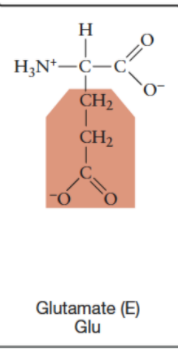
\includegraphics[width=.9\linewidth]{./Screen Shot 2020-09-16 at 2.57.31 PM.png}
\caption{Screen Shot 2020-09-16 at 2.57.31 PM.png}
\end{figure}

The White parts => "Backbone" aforementioned

The Orange parts => "Sidechain"

A small chain of amino acids are called "peptide". Put many of those
together and you get a\ldots{}

\subsection{Protein!}
\label{sec:orgc4c2382}
\href{KBhBIO101Proteins.org}{KBhBIO101Proteins} are important
biological structures formed by dehydrating multiple amino acids
together.

\subsection{Polymerization}
\label{sec:org93b975f}
The process by which Amino Acids get chained together to make
\href{KBhBIO101Proteins.org}{KBhBIO101Proteins} is called
"Polymerization via Dehydration."

Take two amino acids, take the H-O out of the alcahol, take the H out of
the Amine. Fill the hole with the other one
\end{document}
